%%%%%%%%%%%%%%%%%%%%%%%%%%%%%%%%%%%%%%%%%
% Reporte de prácticas
% Ingeniería Informática
% LaTeX Template
% Version 0.1 (27/09/20)
% Original author: Abraham Marianjel Sepúlveda
%%%%%%%%%%%%%%%%%%%%%%%%%%%%%%%%%%%%%%%%%%
\documentclass[12pt,letterpaper]{article} 
\usepackage[utf8]{inputenc} 
\usepackage[spanish, es-tabla, es-nodecimaldot]{babel} % Formato a español
\usepackage[T1]{fontenc}    % Permite utilizar otras tipografías
\usepackage[vmargin=2.5cm,hmargin=2.5cm]{geometry}
\usepackage{multicol}   % Unir columnas en tablas y formato a dos columnas
\usepackage{multirow}   % Unir filas en tablas
\usepackage{graphicx}   % Necesario para insertar gráficas
\usepackage{float}      % Corregir ubicación de imágenes y tablas
%\usepackage{subfigure} % Insertar subfiguras
\usepackage{url}       % Hiervínculo a direcciones URL
\usepackage{cite}
\usepackage{lscape} % Para poner una unica hoja en horizontal
\usepackage{listings}
\usepackage{flushend}
\usepackage[none]{hyphenat} % Permite utilizar el comando \sloppy
\usepackage[small]{caption}	% Reduce el tamaño de letra utilizado en los pies de figura.
\usepackage{hyperref}   % Agrega enlaces internos de las secciones, figuras y tablas.
\usepackage{color}      % Definición de colores
    \hypersetup{colorlinks=true, linkcolor=[rgb]{0,0,1}, citecolor=[rgb]{0,0,1}}
\usepackage{xcolor}		% Permite definir un color para utilizarlo dentro del documento.
    \definecolor{gris}{RGB}{70,70,70}	% Definiendo el color gris
    \definecolor{negro}{RGB}{40,40,40}		% Definiendo el color negro

%%%%%%%% Modificación de los espacios de los títulos de secciones %%%%%%%%%%
%======================================================================================
\usepackage{titlesec}		% Permite reconfigurar  los títulos de las secciones y subsecciones
%\renewcommand\thesection{\Roman{section}}	% Numeración romana en las secciones
\renewcommand\thesubsection{\Roman{subsection}}		% Numeración romana en las subsecciones
\titlespacing*{\section}{0pt}{2.5mm}{0mm}	% Espaciado del título {espacio izquierdo}{arriba del título}{abajo del título}
\titleformat{\section}[block]{\large\scshape\centering}{\thesection.}{1em}{}	% Espaciado del título de las secciones
\titleformat{\subsection}[block]{\large}{\thesubsection.}{1em}{}				% Espaciado del título de las subsecciones
%%%%%%%%%%%%%%%%%%%%%%%%%%%%%%%%%%%%%%%%%%%%%%%%%%%%%%%%%%%%%%%%%%%%%%%%%%%%%%

%Se define un comando \colorhrule para hacer líneas horizontales de color con 3 argumentos: color, largo, ancho.
\newcommand{\colorhrule}[3]{\begingroup\color{#1}\rule{#2}{#3}\endgroup}

\setlength{\intextsep}{1mm} % Distancia superior e inferior en objetos flotantes
\setlength{\columnsep}{5mm} % Separación entre columnas del documento
%**************************************Encabezado****************************************
%=========================================================================================
\begin{document}
\sloppy     % Evita que las palabras se corten al saltar de línea.
\begin{center}
	\begin{tabular}{cc}
	\multirow{2}{3.5cm} {
\includegraphics[scale=0.3]{../../../Logos FACE/logosimbologia.png}   }	& \huge{\textsc{\textbf{Universidad del Bio Bio}}}\\ %\vspace{5mm}
 & \scriptsize{\textsc{Facultad de Ciencias Empresiariales}}\\[4mm]% Sele puede cambiar al LARGE
 & \Large{\textsf{\textbf{Guía Diagrama de Clases}}}\\
 & \small Profesor: {\textsf{Luis Rojas}}\\
 & \small Ayudante: {\textsf{Abraham Marianjel}}\\

 & \small{\textsc{Ingeniería Civil en Informática $|$ Modelamiento}}\\
 & \today\\
	\end{tabular}
\end{center}
\begin{center}
\colorhrule{negro}{16.5cm}{1.2pt}
\end{center}

\begin{abstract}
\noindent \par El diagrama de clases es una técnica central y ampliamente difundida en los distintos
métodos orientados a objeto. Cada método incluye sus propias variantes a esta técnica. 
\end{abstract}
\begin{center}
\vspace{-5mm}
\colorhrule{gris}{16.5cm}{0.7pt}
\end{center}
%*******************************Texto del Informe*********************************************
%==============================================================================================

\par \textsc{Descripción:} \textit{Los diagramas de clase describen los tipos de objetos de un sistema, así como los distintos tipos de relaciones que pueden existir entre ellos. Los diagramas de clase se convierten así en la técnica más potente para el modelado conceptual de un sistema software, la cual suele recoger los conceptos clave del modelo de objetos subyacente al método orientado a objetos que la incorpora,.}\vspace{2cm}

\section*{\LARGE\textbf{Utilidad}}
Se puede decir que existen tres perspectivas diferentes desde las cuales se pueden utilizar los diagramas de clase:

\begin{itemize}
    \item \textit{Conceptual:} El diagrama de clase representa los conceptos en el dominio del problema que se está estudiando. Este modelo debe crearse con la mayor independencia posible de la implementación final del sistema.
    \item \textit{Especificación:} El diagrama de clase refleja las interfaces de las clases, pero no su implementación. Aquí las clases aparecen más cercanas a los tipos de datos, ya que un tipo representa una interfaz que puede tener muchas implementaciones diferentes.
    \item \textit{Implementación:} Esta vista representa las clases tal cual aparecen en el entorno de implementación.
\end{itemize}
\vspace{1cm}

\section*{\LARGE\textbf{Elementos de los diagrama de clases}}
El icono de una clase es un rectángulo dividido en tres secciones, como se puede apreciar en la Figura 1. La sección superior contiene el nombre de la clase, la sección intermedia contiene la lista de atributos, y la sección inferior contiene la lista de operaciones de la clase.\\

	\begin{figure}[H]
		\centering
		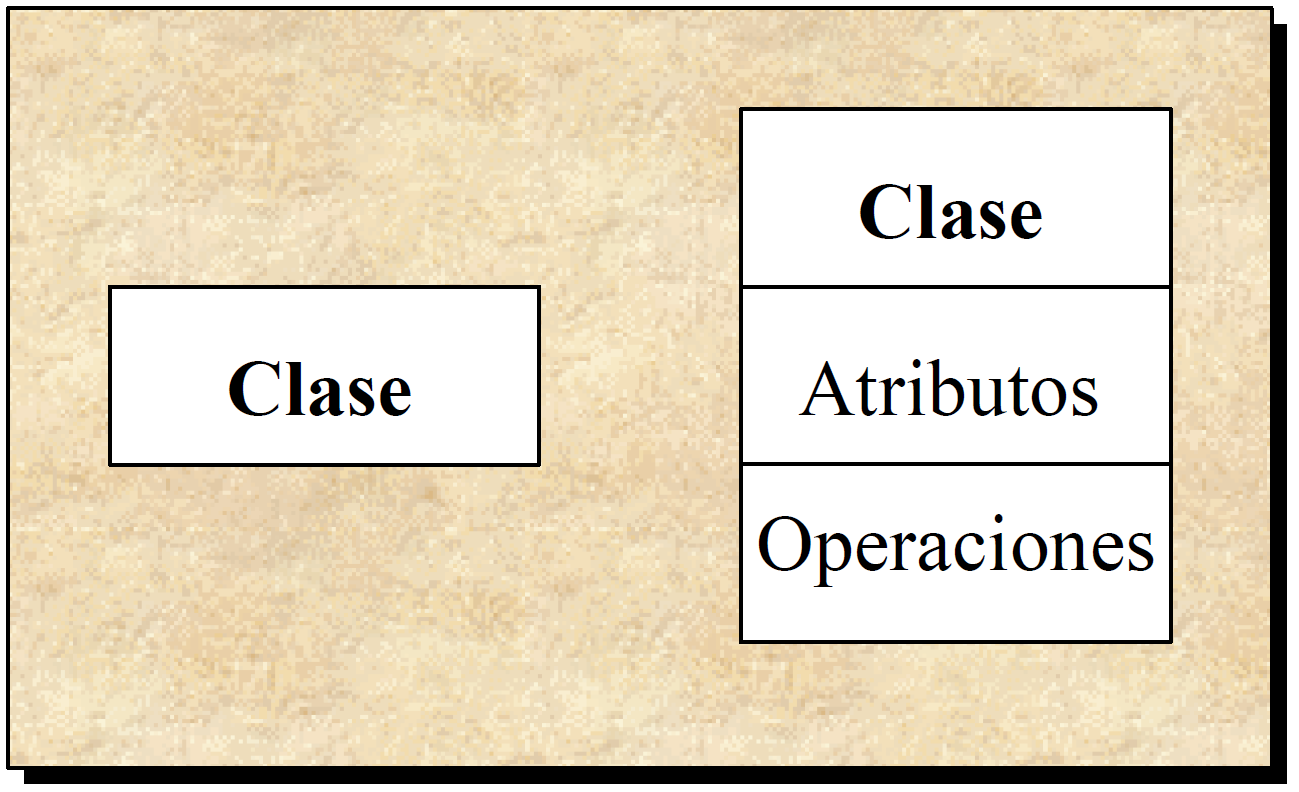
\includegraphics[scale=0.2]{img/clases.PNG}     
		\caption{Representación de Clase }
	\label{fig:rc}
	\end{figure}
	
	\begin{figure}[H]
		\centering
		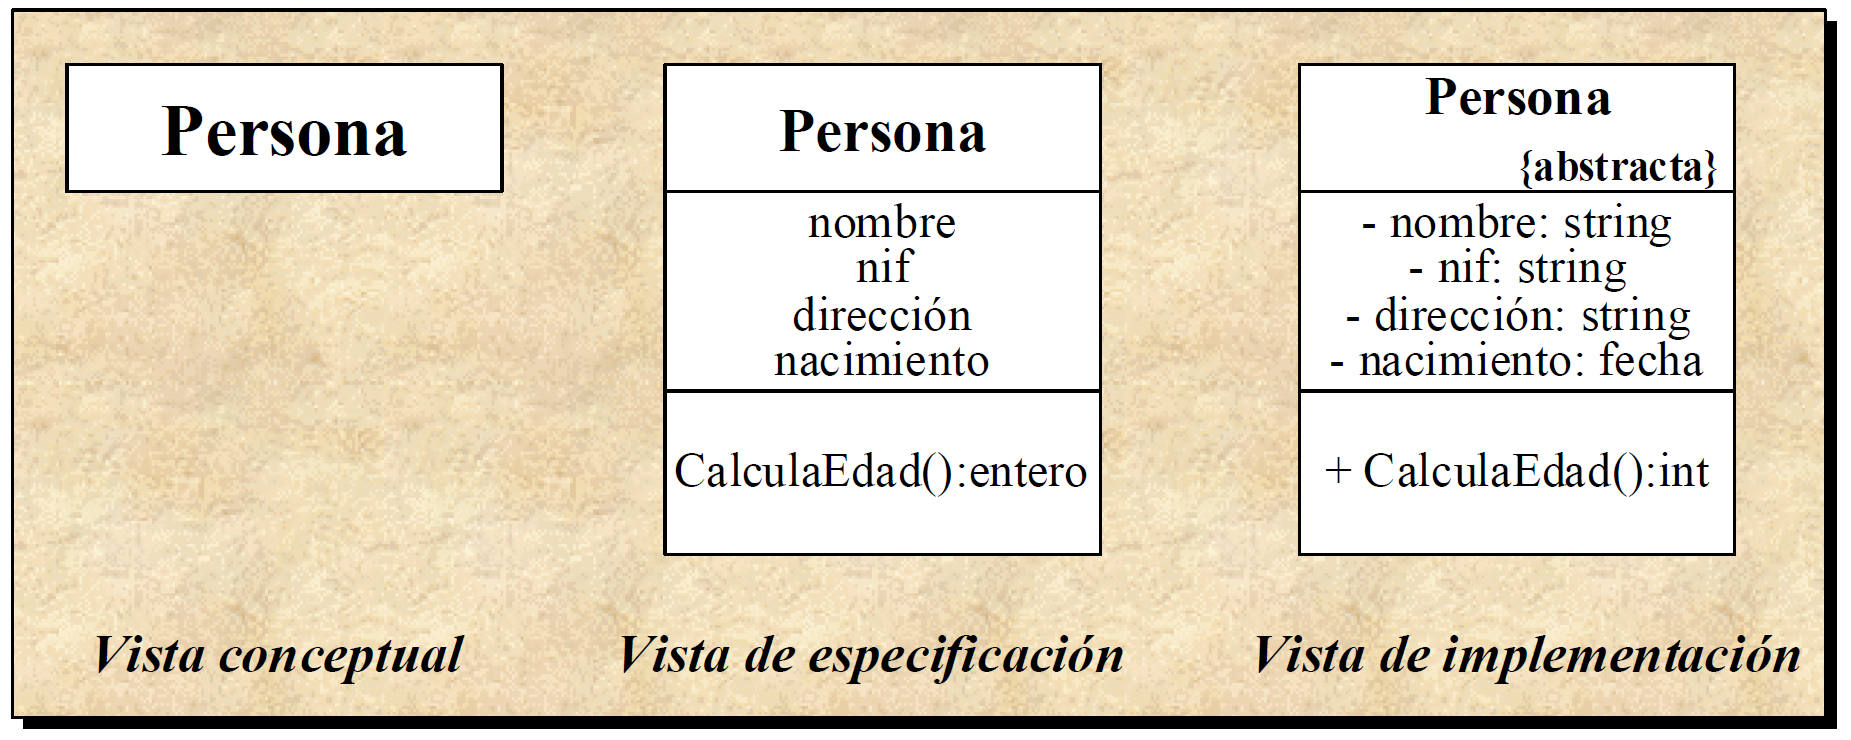
\includegraphics[scale=0.2]{img/vistas de clase.PNG}     
		\caption{Vistas de un diagrama de clases}
	\label{fig:rc}
	\end{figure} \vspace{1cm}
	
Las \textbf{asociaciones} representan las relaciones entre clases, las asociaciones son por defecto bidireccionales, de forma que cuando se quiera modelar una asociación unidireccional entre clases, debe indicarse de forma explícita.\\ 

	\begin{figure}[H]
		\centering
		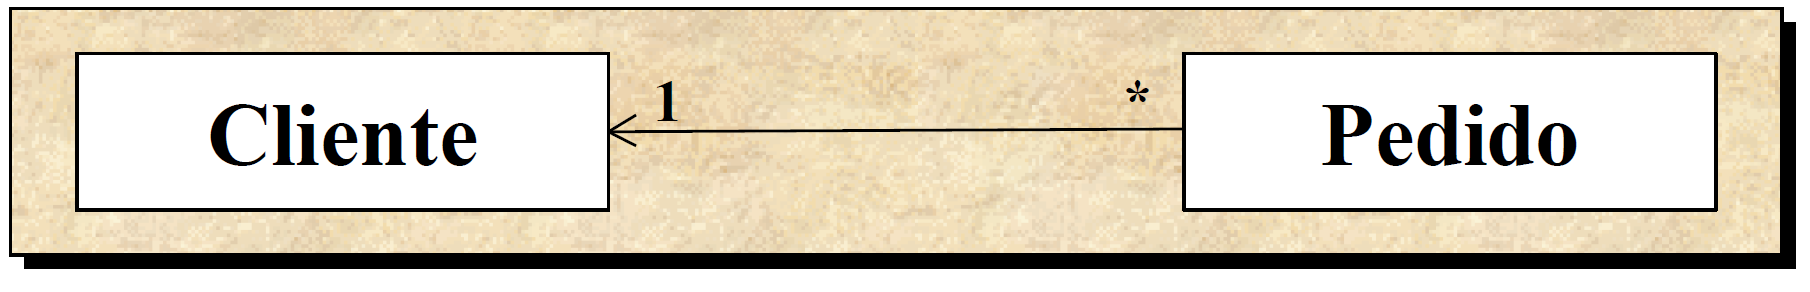
\includegraphics[scale=0.2]{img/asociacion.PNG}      
		\caption{Asociación}
	\label{fig:rc}
	\end{figure}
	\vspace{1cm}

La \textbf{agregación} es una asociación con unas connotaciones semánticas más definidas: la agregación es la relación parte-de, que presenta a una entidad como un agregado de partes (en orientación a objeto, un objeto como agregado de otros objetos).

	\begin{figure}[H]
		\centering
		\includegraphics[scale=0.2]{img/agregación.PNG}       
		\caption{Asociación}
	\label{fig:rc}
	\end{figure}
	\vspace{1cm}
	
La \textbf{composición} implica que los componentes de un objeto sólo pueden pertenecer a un solo objeto agregado, de forma que cuando el objeto agregado es destruido todas sus partes son destruidas también.\\
	\begin{figure}[H]
		\centering
		\includegraphics[scale=0.2]{img/composición.PNG}     
		\caption{Composición}
	\label{fig:rc}
	\end{figure}
	\vspace{1cm}

La \textbf{herencia} es la típica relación de generalización/especialización entre clases. En UML la herencia se representa mediante una flecha, cuya punta es un triángulo vacío. La flecha que representa a la herencia va orientada desde la subclase a la superclase.\\
	\begin{figure}[H]
		\centering
		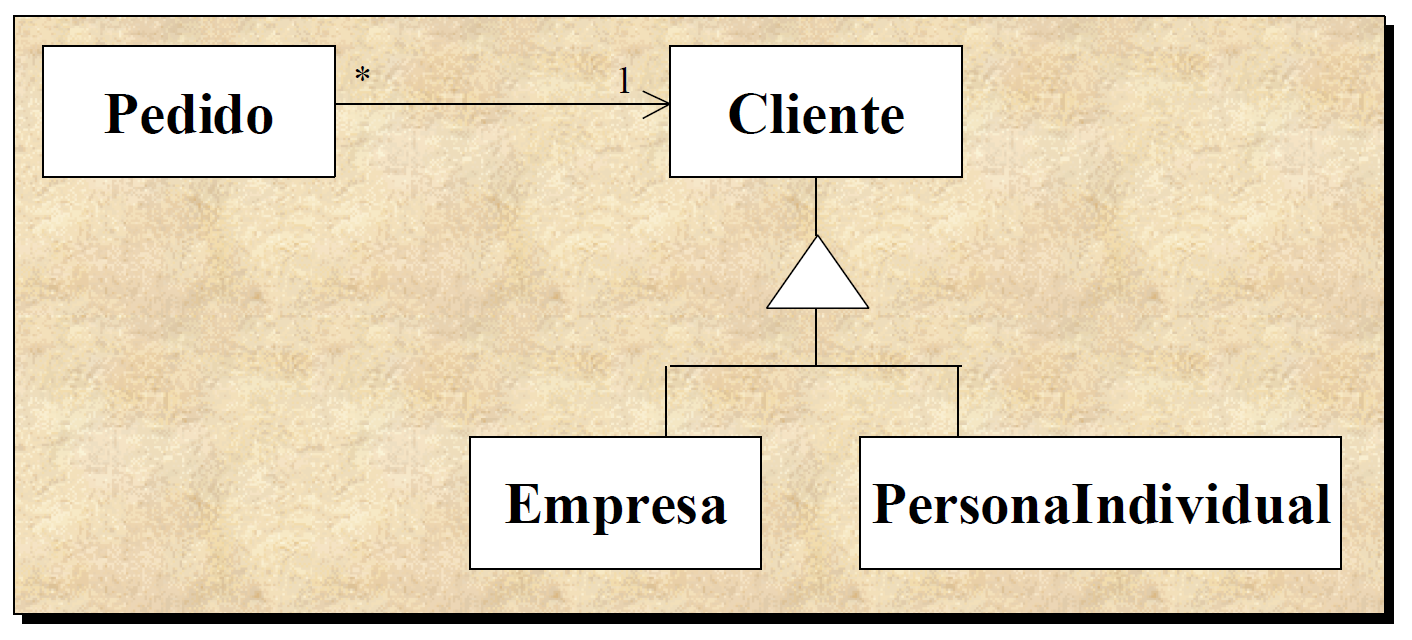
\includegraphics[scale=0.2]{img/herencia.PNG}     
		\caption{Herencia}
	\label{fig:rc}
	\end{figure}
	\vspace{1cm}
	
La Figura 6 muestra un caso en el que los pedidos pueden ser realizados por dos tipos de clientes: una empresa o una persona individual. Según esto, la clase Cliente es una generalización de las clases Empresa y PersonaIndividual, o visto en la otra dirección, Empresa y PersonaIndividual son especializaciones de Cliente.\\


\section*{\LARGE\textbf{ Actividades}}
\textit{En las actividades a desarrollar esta la replicación y la interpretación del proceso de negocios, modelandolo con herramientas digitales o en su cuaderno.}\\

\subsection{\textbf{McDonals}}
Relacionar en un diagrama de clases los terminos:
El cliente posee muchos pedidos a MacDonals y MacDonls tiene muchos clientes, además McDonals tiene muchos productos que son de muchos distribuidores. Los clientes solo trabajan en un lugar. Mcdonals tiene muchas sucursales y empleados.\\

\subsection{\textbf{Bicicleta}}
Represente un diagrama de clases con los términos mencionados anteriormente (Agregación, composición, herencia, asociación).\\


\subsection{\textbf{Persona}}
Redactar lo que pasa en el diagrama de clases:
	\begin{figure}[H]
		\centering
		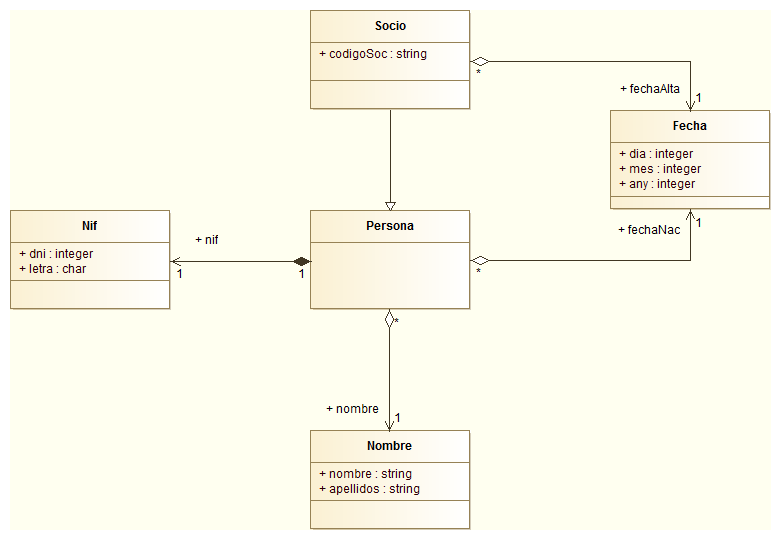
\includegraphics[scale=0.4]{img/personaUML.png}      
		\caption{Herencia}
	\label{fig:rc}
	\end{figure}
	\vspace{1cm}


\subsection{\textbf{Cajero automático}}
Se ha de realizar el diagrama de clases con la siguiente información.
\par Una familia desea obtener dinero, por que en el negocio Don Juanito no aceptar tarjetas bancarias, para eso la familia debe recurrir a un cajero automático para retirar dinero. \\

\subsection{\textbf{Empleados de una empresa}}
Represente mediante diagrama de clases la siguiente necesidad:
Una aplicación necesita almacenar información sobre empresas, sus empleados y sus clientes. Ambos se caracterizan por su nombre y edad.
\par Los empleados tienen un sueldo bruto, los empleados directivos tienen una categoria, asi como un conjunto de empleados subordinados.
\par De los clientes además se necesita conocer su teléfono de contacto.
\par \textit{La aplicación necesita mostrar los datos de empleado y clientes.}\\


\subsection{\textbf{Proyecto}}
Un estudio de arquitectura desea crear una base de datos para gestionar sus proyectos. Nos dan las siguientes especificaciones: 
\par Cada proyecto tiene un código y un nombre. Un proyecto tiene uno y solo un jefe de proyecto y un jefe de proyecto sólo puede estar involucrado en un proyecto o en ninguno. 
\par De cada jefe de proyecto se desean recoger sus datos personales (código, nombre, dirección y teléfono). Un jefe de proyecto se identifica por un código. No hay dos nombres de jefe de proyecto con el mismo nombre. 
\par Un proyecto se compone de una serie de planos, pero éstos se quieren guardar de modo independiente al proyecto. Es decir, si en un momento dado se dejara de trabajar en un proyecto, se desea mantener la información de los planos asociados. 
\par De los planos se desea guardar su número de identificación, la fecha de entrega, los arquitectos que trabajan en él y un dibujo del plano general con información acerca del número de figuras que contiene. 
\par Los planos tienen figuras. De cada figura se desea conocer, el identificador, el nombre, el color, el área y el perímetro. Además, de los polígonos se desea conocer el número de líneas que tienen, además de las líneas que lo forman. El perímetro se desea que sea un método diferido; el área se desea implementarlo como genérico para cualquier tipo de figura, pero además se desea un método específico para el cálculo del perímetro de los polígonos. 
\par De cada líneas que forma parte de un polígono se desea conocer el punto de origen y el de fin (según sus coordenadas, X e Y), así como la longitud. Cada línea tiene un identificador que permite diferenciarlo del resto. La longitud de la línea se puede calcular a partir de sus puntos origen y final.\\

'
\end{document}
